%% Springer Nature journal article template (sn-jnl, v3.1) -- manuscript
%% Reference style: Basic Springer Nature (sn-basic), author-year
\documentclass[pdflatex,sn-basic]{sn-jnl}

\usepackage{graphicx}%
\usepackage{multirow}%
\usepackage{amsmath,amssymb,amsfonts}%
\usepackage{amsthm}%
\usepackage{mathrsfs}%
\usepackage[title]{appendix}%
\usepackage{xcolor}%
\usepackage{textcomp}%
\usepackage{manyfoot}%
\usepackage{booktabs}%
\usepackage{algorithm}%
\usepackage{algorithmicx}%
\usepackage{algpseudocode}%
\usepackage{listings}%

\theoremstyle{thmstyleone}%
\newtheorem{theorem}{Theorem}%
\newtheorem{proposition}[theorem]{Proposition}%
\theoremstyle{thmstyletwo}%
\newtheorem{example}{Example}%
\newtheorem{remark}{Remark}%
\theoremstyle{thmstylethree}%
\newtheorem{definition}{Definition}%

\raggedbottom

\newcommand{\fitpaper}{\mathrm{fit}_{\mathrm{paper}}}
\newcommand{\fitQA}{\mathrm{fit}_{\mathrm{QA}}}
\newcommand{\fitFA}{\mathrm{fit}_{\mathrm{FA}}}

\begin{document}

\title[Queue-Aware and Failure-Aware Fitness for QoS-MDPSO]{Queue-Aware and Failure-Aware Fitness for Multi-Objective PSO Cloud Scheduling: Replication, Ablation and Failure Analysis of QoS-MDPSO}

\author*[1]{\fnm{Vatsal} \sur{Sharma}}\email{mail2vatsalsharma@gmail.com}
\equalcont{These authors contributed equally to this work.}
\author[1]{\fnm{Harshit}}\email{Harshit.workcompany@gmail.com}
\equalcont{These authors contributed equally to this work.}
\author[1]{\fnm{Kanishk} \sur{Gupta}}\email{gkanishk266@gmail.com}
\equalcont{These authors contributed equally to this work.}

\affil[1]{\orgdiv{Department of Information Technology}, \orgname{Netaji Subhas University of Technology, Main Campus}, \orgaddress{\city{Delhi}, \country{India}}}

\abstract{Task scheduling on Infrastructure-as-a-Service clouds is a constrained multi-objective problem in which the finish time, the rental cost and the reliability of a schedule must be balanced under per-task deadlines and budgets. Ouyang and Zhang (2025) proposed QoS-MDPSO, a discrete particle swarm optimizer that minimizes makespan and cost and maximizes total credibility. We re-implemented it together with its baselines (DPSO and Min-Min) and examined its model in detail. Its deadline test ignores queueing on a single-core virtual machine: at the default setting it reports 0.6 missed deadlines where 37.6 of 100 tasks actually finish late. We identify six further issues in its fitness function, search mechanisms and reporting. We contribute (i) a queue-aware evaluator that executes the tasks of every VM in earliest-deadline-first order; (ii) QA-QoS-MDPSO, which keeps the search unchanged and replaces only the fitness with a queue-aware, normalized, additively penalized one; (iii) a one-at-a-time ablation of the five QoS-MDPSO mechanisms with evaluation-count accounting; and (iv) a Monte Carlo failure model in which credibility is the per-attempt success probability, together with a failure-aware fitness (FA-QoS-MDPSO). Over ten seeds per setting, QA-QoS-MDPSO reduces true deadline misses by 27.4\% and 58.9\% (task-length and task-count sweeps) and makespan by 5.6\% and 17.1\% relative to QoS-MDPSO, but lowers total credibility by 8.3\% and 11.7\%. Credibility strongly predicts task survival under failures (Pearson $r=0.889$); FA-QoS-MDPSO completes the most tasks (84.3\% against 78.8\% for QoS-MDPSO). We also report results unfavorable to the original method: a textbook Min-Min beats every PSO variant on makespan and true deadline misses, one mechanism (spbest) degrades the original fitness, and QoS-MDPSO uses three times the evaluation budget of DPSO.}

\keywords{Cloud task scheduling, Particle swarm optimization, Deadline and budget constraints, Queue-aware evaluation, Credibility, Failure-aware scheduling, Ablation, Reproducibility}

\maketitle

%% ------------------------------------------------------------------
\section{Introduction}\label{sec1}
%% ------------------------------------------------------------------
Infrastructure-as-a-Service (IaaS) clouds let users rent virtual machines (VMs) by the hour instead of owning hardware \citep{mell2011}. Rented VMs differ in processing speed, hourly price and reliability, and a scheduler must decide which VM executes each submitted task. That single decision fixes when the workload finishes, what it costs and how likely it is to fail. These goals conflict: faster VMs cost more per hour, and the most reliable VM is not necessarily the fastest. Task scheduling is therefore a constrained multi-objective optimization problem.

The problem is also combinatorially hard. With $n$ tasks and $m$ VMs there are $m^{n}$ possible assignments; for the 100 tasks and 12 VMs of our default setting this is about $10^{108}$, more than the number of atoms in the observable universe. Scheduling independent tasks on heterogeneous machines is NP-hard \citep{garey1979,ibarra1977}, so exact methods do not scale, and meta-heuristics such as genetic algorithms, ant colony optimization and particle swarm optimization (PSO) \citep{kennedy1995} are widely used to find good schedules in reasonable time \citep{houssein2021}.

Ouyang and Zhang \citeyearpar{ouyang2025} recently proposed QoS-MDPSO (Quality-of-Service-guided Multi-objective Discrete PSO). It minimizes makespan and total execution cost and maximizes total credibility, subject to a deadline and a budget for every task. On top of standard discrete PSO it adds five mechanisms: a chaotic non-linear inertia weight, diversity-enhanced personal-best learning (spbest), a population-mean ``mainstream'' attractor (mbest), an adaptive position update and replacement of the worst particle. Against DPSO the authors report a 19.69\% shorter makespan, 4.39\% lower cost and 7.04\% higher total credibility in a task-length experiment, and 14.08\%, 2.74\% and 2.89\% in a task-count experiment.

The central claim of \citet{ouyang2025} is that its schedules complete tasks on time and within budget. Its deadline test (Eq.~9 of \citet{ouyang2025}), however, compares each task's \emph{execution time} with its deadline. Every VM in the model has a single processing unit, so tasks assigned to the same VM run one after another and a task's \emph{completion time} includes the time it spends waiting. A schedule can pass Eq.~9 for every task and still miss most deadlines. In addition, the fitness function (Eq.~11 of \citet{ouyang2025}) sums hours, dollars and a unitless credibility score with fixed weights, and enters the constraints only through a divisor that lies between 1 and 2.

This work began as a reproduction of \citet{ouyang2025} for a cloud computing course and grew into an analysis of its model. We ask four research questions:
\begin{enumerate}
\item[\textbf{RQ1}] Can the main claims of \citet{ouyang2025} be reproduced independently?
\item[\textbf{RQ2}] How large is the gap between the paper's deadline check and the true, queue-aware deadline misses, and does a queue-aware fitness close it?
\item[\textbf{RQ3}] Which of the five QoS-MDPSO mechanisms actually contribute?
\item[\textbf{RQ4}] Does credibility predict surviving VM failures, and can a failure-aware fitness do better?
\end{enumerate}

\textbf{Contributions.} (1) A seeded, open reimplementation of the environment, DPSO, Min-Min and QoS-MDPSO in which every parameter is labelled as taken from \citet{ouyang2025} or assumed. (2) An analysis identifying seven issues in \citet{ouyang2025}, chief among them the queue-blind deadline test. (3) QA-QoS-MDPSO, a queue-aware normalized fitness that leaves the search unchanged. (4) A per-mechanism ablation with evaluation-count accounting. (5) A failure model that gives credibility an operational meaning, and FA-QoS-MDPSO, a failure-aware fitness. Negative and mixed results are reported alongside positive ones. The complete source code, data and scripts are available in the project repository (Section~\ref{sec:avail}).

The rest of the paper is organized as follows. Section~\ref{sec2} reviews background and related work. Section~\ref{sec3} describes the system model and the base algorithm. Section~\ref{sec4} analyses the issues in the base paper with a worked example. Section~\ref{sec5} presents our methods, Section~\ref{sec6} the implementation and experimental setup, and Section~\ref{sec7} the results. Section~\ref{sec8} discusses the findings and their limitations and Section~\ref{sec9} concludes.

%% ------------------------------------------------------------------
\section{Background and related work}\label{sec2}
%% ------------------------------------------------------------------
\subsection{Heuristics for independent tasks}\label{sec2.1}
The classic list heuristics for mapping independent tasks onto heterogeneous machines are Min-Min and Max-Min \citep{ibarra1977,maheswaran1999}. Min-Min keeps a ready time for every machine and repeatedly schedules the unscheduled task whose earliest possible completion time is smallest, on the machine that achieves it. Max-Min instead schedules the task whose earliest completion time is largest, which tends to place long tasks first. In a well-known comparison of eleven static mapping heuristics, Min-Min was among the strongest fast methods for makespan \citep{braun2001}. For dependent tasks (workflows), HEFT \citep{topcuoglu2002} and PEFT \citep{arabnejad2014} rank tasks by their critical-path position and assign them to the processor with the earliest finish time. These heuristics run in milliseconds but optimize only time; they ignore cost, reliability and per-task constraints.

\subsection{Particle swarm optimization and its variants}\label{sec2.2}
PSO \citep{kennedy1995} maintains a swarm of candidate solutions (particles). Each particle has a position and a velocity, remembers the best position it has found (\emph{pbest}) and knows the best position found by the swarm (\emph{gbest}). At every iteration the velocity is updated as $v \leftarrow w v + c_1 r_1(\mathit{pbest}-x) + c_2 r_2(\mathit{gbest}-x)$ and the position as $x \leftarrow x+v$, where $r_1,r_2$ are random numbers in $[0,1]$. The inertia weight $w$ balances exploration and exploitation; a weight that decreases over time was introduced in \citep{shi1998}, and constriction coefficients were analysed in \citep{clerc2002}. A known weakness is premature convergence: the swarm collapses onto gbest early and stalls in a local optimum. Many variants change the inertia schedule or the learning targets to delay this. Adaptive PSO \citep{zhan2009} adjusts the inertia weight and acceleration coefficients according to the evolutionary state of the swarm, dimensional-learning PSO \citep{xu2019} builds the learning exemplar dimension by dimension, and the adaptive strategies of \citep{liu2020} are the direct source of several QoS-MDPSO equations (chaotic inertia weight, diversity-enhanced learning and mainstream learning). A systematic review of PSO and its applications is given in \citep{gad2022}.

\subsection{Discrete PSO for scheduling}\label{sec2.3}
A schedule is a vector of machine choices, not a point in continuous space. Discrete variants include binary PSO \citep{kennedy1997}, in which velocity sets the probability of a bit flip; rounding continuous positions to the nearest machine index; and permutation or swap-based encodings. QoS-MDPSO uses an integer encoding in which entry $i$ is the VM index of task $i$, with velocities limited to $[-m/2,m/2]$. The paper does not state how fractional positions are converted to indices; we round and clip.

\subsection{Cloud task scheduling: a literature review}\label{sec2.4}
Houssein et al.\ \citeyearpar{houssein2021} survey meta-heuristic cloud task scheduling and classify methods by their objectives. We organize the closest work around the three QoS attributes of QoS-MDPSO.

\textit{Makespan-oriented methods.} Khalili and Babamir \citeyearpar{khalili2015} use PSO with a linear inertia weight to shorten the makespan of dynamic cloud scheduling. Alruwais et al.\ \citeyearpar{alruwais2024} propose a farmland-fertility-based algorithm that balances load across resources, and Laha et al.\ \citeyearpar{laha2024} propose an enhanced shortest-job-first scheme with priorities that sends long tasks to powerful VMs. Learning-based methods are increasingly common: QL-HEFT \citep{tong2020} combines Q-learning with HEFT, Ding et al.\ \citeyearpar{ding2020} use Q-learning with an M/M/S queue model to reduce energy, and Amini and Kalbasi \citeyearpar{amini2024} apply deep Q-learning to learn near-optimal policies from the system state.

\textit{Cost- and deadline-oriented methods.} Zuo et al.\ \citeyearpar{zuo2013} schedule independent tasks on hybrid IaaS clouds with a self-adaptive learning PSO under deadline constraints, with the aim of raising provider profit. For workflows, Wu et al.\ \citeyearpar{wu2017} propose ProLiS and L-ACO, which distribute the deadline over tasks and minimize cost, and Ye et al.\ \citeyearpar{ye2024} extend this to IoT workflows with deadline and budget constraints. Rodriguez and Buyya \citeyearpar{rodriguez2014} study deadline-based provisioning and scheduling for scientific workflows.

\textit{Trust- and reliability-aware methods.} Rjoub et al.\ \citeyearpar{rjoub2020} compute a trust level for each VM and use it to prioritize big-data tasks, while Choppara and Mangalampalli \citeyearpar{choppara2024} combine trust and reliability awareness with an actor-critic reinforcement-learning scheduler for cloud--fog systems. In these works credibility or trust is a modelled score; it is not validated against simulated failures, which is the gap we address in Section~\ref{sec5.3}.

\textit{Multi-objective deadline- and budget-constrained methods.} Panda and Jana \citeyearpar{panda2015} and Zuo et al.\ \citeyearpar{zuo2016} balance makespan and cost for independent tasks on multi-cloud systems, the latter also under deadline and cost constraints. For workflows, Kalra and Singh \citeyearpar{kalra2019} combine intelligent water drops with a genetic algorithm to optimize time and reliability, Calzarossa et al.\ \citeyearpar{calzarossa2021} treat deadlines and budgets probabilistically in uncertain clouds, Gupta et al.\ \citeyearpar{gupta2021} add user-defined weights and credibility to a Jaya-based scheduler, and Zhou et al.\ \citeyearpar{zhou2023} control cost through task-level budgets. Ouyang and Zhang \citeyearpar{ouyang2025} are, to our knowledge, the first among these to optimize makespan, cost and credibility simultaneously for independent tasks with PSO. Multi-objective evolutionary algorithms such as NSGA-II \citep{deb2002} instead return a Pareto front, whereas QoS-MDPSO scalarizes the three objectives into a single weighted fitness, which is the design we keep.

Table~\ref{tab:lit} summarizes the related work. Two observations motivate this study. First, most deadline-constrained work evaluates feasibility on the task's own execution time or on a sub-deadline; the effect of queueing on a sequential machine is rarely examined, even though completion-time lateness is classical in single-machine scheduling \citep{jackson1955}. Second, credibility is treated as an objective to maximize without checking whether it predicts anything observable.

\begin{table}[!t]
\caption{Summary of related work on cloud task scheduling (T = task type: I independent, W workflow)}\label{tab:lit}
\footnotesize
\setlength{\tabcolsep}{3pt}
\begin{tabular}{@{}p{2.9cm}cp{3.0cm}p{3.7cm}@{}}
\toprule
Work & T & Method & Objectives / constraints\\
\midrule
Khalili and Babamir \citeyearpar{khalili2015} & I & PSO, linear inertia & Makespan\\
Alruwais et al.\ \citeyearpar{alruwais2024} & I & Farmland fertility & Makespan, load balance\\
Laha et al.\ \citeyearpar{laha2024} & I & Enhanced SJF with priority & Makespan\\
Tong et al.\ \citeyearpar{tong2020} & I & Q-learning + HEFT & Makespan\\
Ding et al.\ \citeyearpar{ding2020} & I & Q-learning, M/M/S & Energy\\
Amini and Kalbasi \citeyearpar{amini2024} & I & Deep Q-learning & Makespan\\
Zuo et al.\ \citeyearpar{zuo2013} & I & Self-adaptive learning PSO & Provider profit, deadline\\
Wu et al.\ \citeyearpar{wu2017} & W & ProLiS, L-ACO & Cost, deadline\\
Ye et al.\ \citeyearpar{ye2024} & W & F-ACO & Cost, deadline, budget\\
Rjoub et al.\ \citeyearpar{rjoub2020} & I & Trust-aware priorities & Trust\\
Choppara and Mangalampalli \citeyearpar{choppara2024} & I & Actor-critic RL & Trust, reliability\\
Panda and Jana \citeyearpar{panda2015} & I & Multi-objective tabu search & Makespan, cost\\
Zuo et al.\ \citeyearpar{zuo2016} & I & Multi-objective ACO & Makespan, cost, deadline\\
Kalra and Singh \citeyearpar{kalra2019} & W & IWD + GA & Time, reliability, deadline, budget\\
Calzarossa et al.\ \citeyearpar{calzarossa2021} & W & Monte Carlo + GA & Makespan, cost, probabilistic constraints\\
Gupta et al.\ \citeyearpar{gupta2021} & W & Jaya, user weights & Makespan, cost, credibility\\
Zhou et al.\ \citeyearpar{zhou2023} & W & BDCWS & Makespan, cost, budget, deadline\\
Ouyang and Zhang \citeyearpar{ouyang2025} & I & QoS-MDPSO & Makespan, cost, credibility, deadline, budget\\
\textbf{This work} & I & QA-/FA-QoS-MDPSO & As above, with queue-aware deadlines and failure-aware credibility\\
\bottomrule
\end{tabular}
\end{table}

\subsection{Constraint handling, deadlines and simulation}\label{sec2.5}
Meta-heuristics usually handle constraints by penalizing the objective. Deb \citeyearpar{deb2000} showed that feasibility rules, in which any feasible solution beats any infeasible one, avoid the tuning problems of weak or unbounded penalties. For deadlines, single-machine scheduling theory measures lateness by completion time, which includes the processing time of every job ahead in the queue; earliest-deadline-first (EDF) ordering minimizes the maximum lateness on one machine \citep{jackson1955}. A deadline model for a sequential VM must therefore account for queueing.

CloudSim \citep{calheiros2011} is the most widely used cloud simulator, but static independent-task models such as that of \citet{ouyang2025} are commonly evaluated with custom simulators; the authors of \citet{ouyang2025} used their own Java program. Their workload follows the Google cloud jobs dataset \citep{hussain2018} and their VM templates follow \citep{guo2017}. Completion-time deadlines and reliability-aware scheduling are established ideas, and we do not claim them as new. Our contribution is to show that a recent peer-reviewed algorithm uses a queue-blind deadline model, to measure the consequences, to correct it inside the optimizer, to test the algorithm's components individually and to evaluate its credibility objective under actual failures.

%% ------------------------------------------------------------------
\section{System model and base algorithm}\label{sec3}
%% ------------------------------------------------------------------
\subsection{Tasks, VMs and objectives}\label{sec3.1}
We adopt the model of \citet{ouyang2025} unchanged so that results are comparable. A batch of $n$ independent tasks is known in advance; task $t_i=\{l_i,d_i,b_i,f_i\}$ has length $l_i$ in million instructions (MI), deadline $d_i$ in seconds, budget $b_i$ in dollars and criticality $f_i\in[0,1]$. There are $m$ VMs; $vm_j=\{\mathrm{MIPS}_j,P_j,F_j\}$ has speed $\mathrm{MIPS}_j$, price $P_j$ per hour and credibility $F_j\in[0,1]$. Each VM has one processing unit. Executing task $i$ on VM $j$ takes and costs
\begin{equation}
e_{ij}=\frac{l_i}{\mathrm{MIPS}_j},\qquad c_{ij}=e_{ij}\cdot P_j .
\label{eq:eij}
\end{equation}
A schedule $x$ assigns each task to one VM ($x_i=j$ means task $i$ runs on $vm_j$). The three objectives of \citet{ouyang2025} are the makespan (the busy time of the most loaded VM), the total execution cost and the total credibility:
\begin{equation}
\mathrm{MS}=\max_{j}\sum_{i:\,x_i=j}e_{ij},\qquad
\mathrm{TEC}=\sum_{i=1}^{n}c_{i,x_i},\qquad
\mathrm{TC}=\sum_{i=1}^{n}f_i\,F_{x_i}.
\label{eq:obj}
\end{equation}
Makespan and cost are minimized; credibility is maximized, rewarding schedules that put important tasks on reliable VMs. Table~\ref{tab:notation} summarizes the notation.

\begin{table}[!t]
\caption{Notation}\label{tab:notation}
\footnotesize
\begin{tabular}{@{}ll@{}}
\toprule
Symbol & Meaning\\
\midrule
$n,\ m$ & Number of tasks, number of VMs\\
$l_i,d_i,b_i,f_i$ & Length (MI), deadline (s), budget (\$), criticality of task $i$\\
$\mathrm{MIPS}_j,P_j,F_j$ & Speed, price per hour, credibility of VM $j$\\
$e_{ij},\ c_{ij}$ & Execution time and cost of task $i$ on VM $j$\\
$C_i$ & Completion time of task $i$ including queueing\\
$\mathrm{MS},\mathrm{TEC},\mathrm{TC}$ & Makespan, total execution cost, total credibility\\
$M_D,\ M_B$ & Deadline and budget violations (Eqs.~9, 10 of \citet{ouyang2025})\\
$M_D^{\mathrm{true}}$ & Deadline violations by completion time (ours)\\
$\alpha,\beta,\gamma,\lambda$ & Objective weights; penalty weight (ours)\\
$N,\ T_{\max}$ & Swarm size, number of iterations\\
$K,\ a_j,\ q_j$ & Maximum attempts; expected attempts and loss probability on VM $j$\\
\bottomrule
\end{tabular}
\end{table}

\subsection{Constraints and fitness of the base paper}\label{sec3.2}
Each task must meet its deadline and its budget. In \citet{ouyang2025} these are written as
\begin{equation}
e_{ij}=\frac{l_i}{\mathrm{MIPS}_j}\le d_i,\qquad c_{ij}\le b_i,
\label{eq:cons}
\end{equation}
(Eqs.~9 and 10 of \citet{ouyang2025}) and $M_D(x)$, $M_B(x)$ count the tasks violating each. The objectives and constraints are combined into one score to be minimized:
\begin{equation}
\fitpaper(x)=\frac{\alpha\,\mathrm{MS}+\beta\,\mathrm{TEC}-\gamma\,\mathrm{TC}}{1+e^{-\sqrt{M_D+M_B}}},\qquad \alpha+\beta+\gamma=1 .
\label{eq:fitpaper}
\end{equation}
This is the sign-corrected form of Eq.~11 of \citet{ouyang2025}; Section~\ref{sec4} explains the correction.

\subsection{DPSO and QoS-MDPSO}\label{sec3.3}
Both algorithms encode a particle as an $n$-dimensional integer vector of VM indices in $\{0,\dots,m-1\}$. DPSO uses the standard velocity and position updates
\begin{align}
V_i(t+1)&=w(t)V_i(t)+c_1r_1\bigl(\mathit{pbest}_i-X_i(t)\bigr)+c_2r_2\bigl(\mathit{gbest}-X_i(t)\bigr),\label{eq:vel}\\
X_i(t+1)&=X_i(t)+V_i(t+1),\label{eq:pos}
\end{align}
with an inertia weight decreasing linearly from 0.9 to 0.4, $c_1=c_2=2$ and the usual pbest and gbest updates (Eqs.~4--8 of \citet{ouyang2025}). QoS-MDPSO (Algorithm~1 of \citet{ouyang2025}) adds five mechanisms:
\begin{enumerate}
\item \textbf{Chaotic inertia weight} (Eqs.~12--13): $R(t+1)=4R(t)(1-R(t))$ and $w(t)=w_{\min}R(t)+t(w_{\max}-w_{\min})/T_{\max}$.
\item \textbf{Diversity-enhanced learning, spbest} (Eqs.~14--15): each particle learns from the winner of a random two-particle tournament between personal bests when that winner is better than its own pbest.
\item \textbf{Adaptive mainstream learning, mbest} (Eq.~16): the social term uses the mean of all personal bests instead of gbest.
\item \textbf{Adaptive position update} (Eqs.~18--21): with $p=\mathrm{fitness}(X_i)/\overline{\mathrm{fitness}}$, a particle moves by $X+V$ if $p<\mathrm{rand}$ and by $wX+(1-w)V$ otherwise.
\item \textbf{End replacement} (Eqs.~22--24): a candidate $(\mathit{pbest}_i-\mathit{pbest}_j)\cdot\mathrm{rand}+\mathit{gbest}$ replaces the worst personal best if it is better.
\end{enumerate}
Fig.~\ref{fig:flow} shows the resulting loop and Algorithm~\ref{alg:psoloop} lists it in pseudocode. The fitness evaluation step is the only part that differs between QoS-MDPSO and our two variants.

\begin{figure}[!t]
\centering
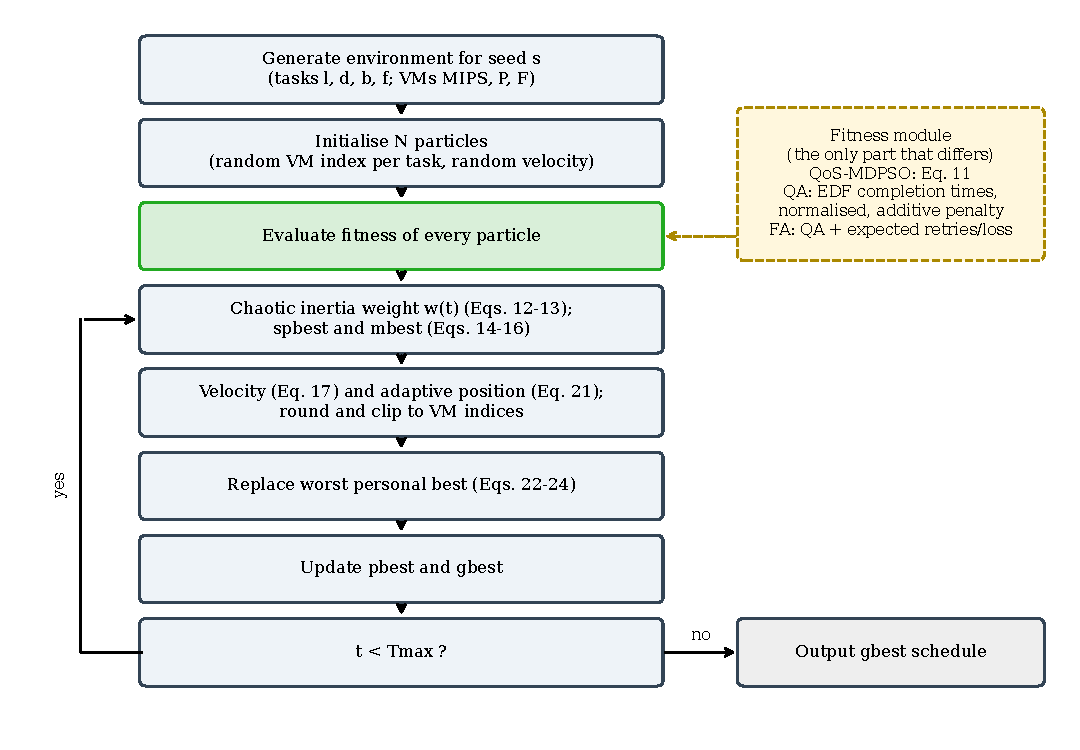
\includegraphics[width=0.78\textwidth]{fig_flow.pdf}
\caption{The QoS-MDPSO loop shared by all PSO variants in this study. QA-QoS-MDPSO and FA-QoS-MDPSO change only the fitness module (dashed box).}\label{fig:flow}
\end{figure}

\begin{algorithm}[!t]
\caption{QoS-MDPSO main loop (fitness module is pluggable)}\label{alg:psoloop}
\begin{algorithmic}[1]
\Require tasks, VMs, swarm size $N$, iterations $T_{\max}$, fitness function \textsc{Fit}
\State Initialise $X_i$ with random VM indices, $V_i$ in $[-m/2,m/2]$; $R(0)\notin\{0,0.25,0.5,0.75,1\}$
\State $\mathit{pbest}_i\leftarrow X_i$; $\mathit{gbest}\leftarrow\arg\min_i \textsc{Fit}(X_i)$
\For{$t=1$ to $T_{\max}$}
  \State $R\leftarrow 4R(1-R)$; $w\leftarrow w_{\min}R+t(w_{\max}-w_{\min})/T_{\max}$
  \State Compute $\mathit{spbest}_i$ (tournament, Eqs.~14--15) and $\mathit{mbest}$ (Eq.~16)
  \For{each particle $i$}
    \State Update $V_i$ (Eq.~17); update $X_i$ by Eq.~21; round and clip to $\{0,\dots,m-1\}$
  \EndFor
  \State Build $\mathit{nbest}$ (Eq.~23); replace the worst personal best if $\textsc{Fit}(\mathit{nbest})$ is lower (Eq.~24)
  \State Update $\mathit{pbest}_i$ and $\mathit{gbest}$ using \textsc{Fit}
\EndFor
\State \Return $\mathit{gbest}$
\end{algorithmic}
\end{algorithm}

%% ------------------------------------------------------------------
\section{Analysis of the base paper}\label{sec4}
%% ------------------------------------------------------------------
\subsection{Worked example: why Eq.~9 misses late tasks}\label{sec4.1}
Consider two VMs, VM1 (200 MIPS) and VM2 (100 MIPS), and three tasks of 400, 200 and 600 MI. On VM1 they take 2, 1 and 3~s; on VM2 4, 2 and 6~s. Suppose VM1 runs T1 then T2 and VM2 runs T3 (Fig.~\ref{fig:example}), and T2 has a deadline of 2.5~s. T2 starts only when T1 finishes, at 2~s, and completes at 3~s, so it is late. Eq.~9 instead checks T2's own execution time, $1\ \mathrm{s}\le 2.5\ \mathrm{s}$, and counts it as on time. The longer a VM's queue, the more tasks are misjudged in this way; the effect grows with the number of tasks and with task length.

\begin{figure}[!t]
\centering
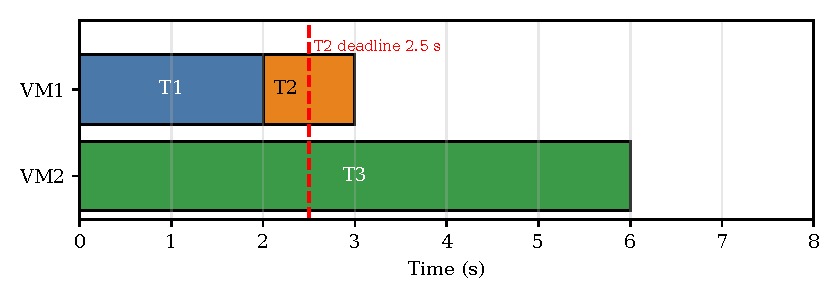
\includegraphics[width=0.62\textwidth]{fig_example.pdf}
\caption{Worked example. T2 waits behind T1 on VM1 and completes at 3~s, after its 2.5~s deadline, yet Eq.~9 of \citet{ouyang2025} counts it as on time because its own execution time is only 1~s.}\label{fig:example}
\end{figure}

The same example shows two properties used later. Even with only $2^3=8$ possible schedules the objectives conflict: the fastest schedule (T2 and T3 on VM1 and T1 on VM2, makespan 4~s) is not the cheapest (everything on VM2). And Min-Min, applied greedily, places all three tasks on VM1 (makespan 6~s), showing that greedy choices need not be optimal on small instances even when, as we will see, they are strong on large ones.

\subsection{Seven issues}\label{sec4.2}
Table~\ref{tab:issues} lists the issues we found in \citet{ouyang2025}. I1 affects the paper's central claim and is the focus of our main contribution; I2 and I3 are fixed by the same new fitness; I5 and I6 are examined by the ablation; I7 is handled by stating every assumption and testing significance.

\begin{table}[!t]
\caption{Issues identified in \citet{ouyang2025} and how this work treats them}\label{tab:issues}
\footnotesize
\setlength{\tabcolsep}{3pt}
\begin{tabular}{@{}llp{3.9cm}p{2.5cm}p{2.1cm}@{}}
\toprule
\# & Where & Issue & Consequence & Treated by\\
\midrule
I1 & Eq.~9 & Deadline compares execution time with $d_i$, ignoring queueing on a single-core VM & Violations under-counted about 60$\times$ at default (0.6 vs 37.6) & Queue-aware evaluator, QA fitness\\
I2 & Eq.~11 & Penalty divisor lies in $[1,2]$; with a negative numerator, violations improve the score & Constraints barely enforced, sometimes rewarded & Additive penalty\\
I3 & Eq.~11 & Hours, dollars and unitless credibility added with equal weights & Weights lose their meaning & Normalization\\
I4 & Eq.~11 & Printed signs minimize credibility; Table~4 of \citet{ouyang2025} shows the corrected form was used & Internal inconsistency & Corrected form used\\
I5 & Eqs.~13, 21 & $w$ rises with $t$, opposite to the text; Eq.~21 swaps the exploration/exploitation rules named in the text & Mechanisms may not act as described & Ablation\\
I6 & Eqs.~16, 18, 23 & VM indices averaged and scaled as numbers; 3$\times$ the fitness evaluations of DPSO & Biased search; unequal budget & Ablation, evaluation counts\\
I7 & Tables 3, 9, 10 & Tables 9 and 10 identical; swarm size, iterations, budgets, weights, runs unreported; no tests & Not exactly reproducible & Stated assumptions, 10 seeds, Wilcoxon\\
\bottomrule
\end{tabular}
\end{table}

\paragraph{I2: a weak and invertible penalty.} The divisor $1+e^{-\sqrt{M_D+M_B}}$ equals 2 with no violations, 1.368 with one, 1.135 with four and practically 1 with 25 or more. A schedule with 100 violations is therefore at most twice as bad as a feasible one. Worse, the numerator $\alpha\mathrm{MS}+\beta\mathrm{TEC}-\gamma\mathrm{TC}$ becomes negative when credibility dominates; dividing a negative number by a smaller divisor makes it more negative, so violations then \emph{improve} the score.

\paragraph{I3: mixed units.} Makespan (about 25~h in our default runs), cost (about \$50) and credibility (about 30, unitless) are added with equal weights, so the term with the largest raw value dominates and the weights lose their stated meaning.

\paragraph{I4: printed signs.} Eq.~11 of \citet{ouyang2025} is printed as $\alpha\mathrm{MS}+\beta\mathrm{TC}-\gamma\mathrm{TEC}$, which would minimize credibility and reward cost. The paper's own Table~4 shows that the corrected form was computed: for task length $2\times10^{6}$ MI, QoS-MDPSO has makespan 11.94, cost 25.26 and credibility 32.04 (Tables 5--7 of \citet{ouyang2025}) and fitness 1.418. The corrected numerator $(11.94+25.26-32.04)/3=1.72$ implies a divisor of 1.21, which is valid. The printed form gives 6.24, which would require a divisor of 4.40, impossible because the divisor never exceeds 2.

\paragraph{I5: mechanisms that contradict their description.} Section~5.3 of \citet{ouyang2025} says the inertia weight should be large early (exploration) and small late (exploitation), but Eq.~13 adds the term $t(w_{\max}-w_{\min})/T_{\max}$, so $w$ rises from about 0--0.4 at the start to 0.5--0.9 at the end. Likewise the text labels Eq.~18 as exploration and Eq.~19 as exploitation and says a particle with $p<\mathrm{rand}$ should explore, yet Eq.~21 applies Eq.~19 when $p<\mathrm{rand}$. We implement the equations as printed and test their effect in the ablation.

\paragraph{I6: encoding and budget.} VM indices are labels, but mbest averages them (VM~0 and VM~2 average to ``VM~1'') and the update $wX+(1-w)V$ shrinks indices toward 0. QoS-MDPSO also evaluates the fitness about three times per particle per iteration (position step, replacement step, best update) against once for DPSO, while the stated complexity $O(T_{\max}\,n\,m)$ omits the swarm size; comparing the two at equal iterations favours QoS-MDPSO.

\paragraph{I7: reporting.} Tables 9 (makespan) and 10 (cost) of \citet{ouyang2025} print identical DPSO and QoS-MDPSO columns, so at least one is a transcription error. Swarm size, iteration count, budget range, objective weights and number of runs are not reported, and no significance tests are given.

%% ------------------------------------------------------------------
\section{Proposed methods}\label{sec5}
%% ------------------------------------------------------------------
Both methods keep every QoS-MDPSO search step (Eqs.~12--24 of \citet{ouyang2025}) and change only the fitness function. Any difference in results is therefore caused by the fitness and not by the search.

\subsection{Queue-aware evaluation}\label{sec5.1}
For each candidate schedule, the tasks on each VM are executed in EDF order \citep{jackson1955}. Task $i$'s completion time $C_i$ is the cumulative execution time of the tasks before it on that VM plus its own, and it is a true deadline miss if $C_i>d_i$. Algorithm~\ref{alg:qa} gives the procedure. All algorithms, including the baselines, are scored with this evaluator; we also report the Eq.~9 count. The evaluator was checked against a brute-force loop. Because EDF minimizes the maximum lateness on a single machine, it is the most favourable fixed ordering for the deadline objective; FIFO order would raise every method's true misses (Section~\ref{sec8.1}).

\begin{algorithm}[!t]
\caption{Queue-aware deadline evaluation}\label{alg:qa}
\begin{algorithmic}[1]
\Require schedule $x$, execution times $e$, deadlines $d$
\State $\mathit{order}\leftarrow$ tasks sorted by deadline (EDF)
\State $\mathit{ready}[j]\leftarrow 0$ for every VM $j$;\quad $M_D^{\mathrm{true}}\leftarrow 0$
\For{$i$ in $\mathit{order}$}
  \State $j\leftarrow x[i]$
  \State $\mathit{ready}[j]\leftarrow \mathit{ready}[j]+e[i][j]$ \Comment{$=C_i$}
  \If{$\mathit{ready}[j]>d[i]$} \State $M_D^{\mathrm{true}}\leftarrow M_D^{\mathrm{true}}+1$ \EndIf
\EndFor
\State \Return $M_D^{\mathrm{true}},\ \max_j \mathit{ready}[j]$ \Comment{misses, makespan}
\end{algorithmic}
\end{algorithm}

\subsection{Queue-aware fitness (QA-QoS-MDPSO)}\label{sec5.2}
Each objective is divided by an instance-specific reference so that all terms are dimensionless and close to 1: $\mathrm{MS}_{\mathrm{lb}}=\sum_i l_i/\sum_j \mathrm{MIPS}_j$, the makespan if all work could be split perfectly; $\mathrm{TEC}_{\mathrm{lb}}=\sum_i\min_j c_{ij}$, every task on its cheapest VM; and $\mathrm{TC}_{\mathrm{ub}}=\sum_i f_i\max_jF_j$, every task on the most credible VM. Violations enter additively as the fraction of violating tasks:
\begin{equation}
\fitQA(x)=\alpha\frac{\mathrm{MS}}{\mathrm{MS}_{\mathrm{lb}}}+\beta\frac{\mathrm{TEC}}{\mathrm{TEC}_{\mathrm{lb}}}+\gamma\Bigl(1-\frac{\mathrm{TC}}{\mathrm{TC}_{\mathrm{ub}}}\Bigr)+\lambda\,\frac{M_D^{\mathrm{true}}+M_B}{n},
\label{eq:fitqa}
\end{equation}
with $\alpha=\beta=\gamma=1/3$ and $\lambda=1$, fixed before the experiments. The penalty can neither saturate nor invert (I2), and the weights now mean what they say (I3). The parameter $\lambda$ lets an operator trade deadline compliance against the other objectives (Section~\ref{sec7.4}). Computing EDF completion times costs one sort per evaluation, $O(n\log n)$; the measured runtime is essentially unchanged (0.198~s against 0.195~s per run in the length sweep).

\subsection{Failure model}\label{sec5.3}
The paper optimizes credibility but never defines what happens when a VM is unreliable. We give it an operational meaning: each execution attempt of a task on VM $j$ succeeds with probability $F_j$. A failure is detected when the attempt ends and the task is re-run on the same VM, paying time and money again, up to $K=3$ attempts; a task failing all attempts is lost, and the tasks queued behind it still run. The number of attempts needed is geometric with parameter $F_j$. For each final schedule we draw 200 random failure scenarios and report the share of tasks completed (also weighted by criticality), lost tasks, lost critical tasks ($f\ge0.7$), the effective makespan and cost including re-runs, and the number of tasks that are lost or finish late.

\subsection{Failure-aware fitness (FA-QoS-MDPSO)}\label{sec5.4}
FA-QoS-MDPSO applies the failure model in expectation inside Eq.~\eqref{eq:fitqa}. The expected number of attempts on VM $j$ and the probability that a task there is lost are
\begin{equation}
a_j=\frac{1-(1-F_j)^{K}}{F_j},\qquad q_j=(1-F_j)^{K}.
\label{eq:aq}
\end{equation}
Every task's execution time and cost are multiplied by $a_j$ of its VM before makespan, cost and completion times are computed, and the expected number of lost tasks $\sum_i q_{x_i}$ is added to the violations in Eq.~\eqref{eq:fitqa}:
\begin{equation}
\fitFA(x)=\fitQA\bigl(x;\ e_{ij}\!\leftarrow\!a_je_{ij},\ c_{ij}\!\leftarrow\!a_jc_{ij}\bigr)+\lambda\,\frac{\sum_{i}q_{x_i}}{n}.
\label{eq:fitfa}
\end{equation}
For example, $F=0.9$ gives $a=1.11$ and $q=0.001$; $F=0.5$ gives $a=1.75$ and $q=0.125$; $F=0.2$ gives $a=2.44$ and $q=0.512$. The optimizer therefore avoids unreliable VMs in proportion to the time, cost and loss they are expected to cause, without an extra objective.

%% ------------------------------------------------------------------
\section{Implementation and experimental setup}\label{sec6}
%% ------------------------------------------------------------------
\subsection{System architecture and implementation}\label{sec6.1}
All algorithms are implemented in Python~3 with NumPy, SciPy, pandas and Matplotlib. The model has no network, hosts or task arrivals, so a custom simulator is sufficient, and evaluating a whole swarm as one array keeps a full run near 0.2~s. For a given seed every algorithm receives the identical environment, so all comparisons are paired. Fig.~\ref{fig:arch} shows the module structure: \texttt{config.py} (all parameters), \texttt{environment.py} (generator and evaluator), \texttt{fitness.py} (paper, QA and FA fitness), \texttt{algorithms.py} (Min-Min, DPSO, QoS-MDPSO with ablation switches), \texttt{failures.py} (Monte Carlo simulator) and the run and analysis scripts. The queue-aware evaluator of Algorithm~\ref{alg:qa} is only a few lines of code:

\begin{figure}[!t]
\centering
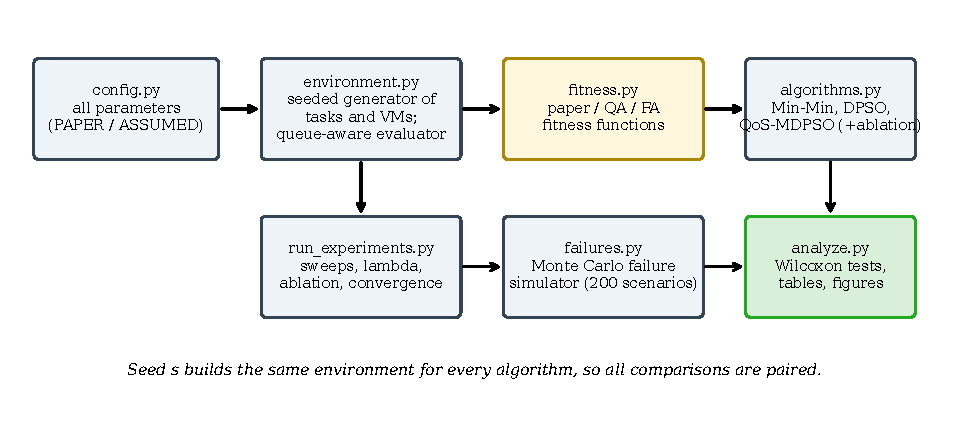
\includegraphics[width=0.85\textwidth]{fig_arch.pdf}
\caption{System architecture of the implementation. The fitness module (highlighted) is the only component that differs between QoS-MDPSO, QA-QoS-MDPSO and FA-QoS-MDPSO.}\label{fig:arch}
\end{figure}

\begin{lstlisting}[basicstyle=\ttfamily\footnotesize,frame=single,language=Python]
def queue_aware(x, e, d, m):
    ready = np.zeros(m)
    misses = 0
    for i in np.argsort(d):          # EDF order
        j = x[i]
        ready[j] += e[i, j]          # completion time C_i
        if ready[j] > d[i]:
            misses += 1
    return misses, ready.max()
\end{lstlisting}

\subsection{Parameters}\label{sec6.2}
Task and VM parameters follow Table~3 of \citet{ouyang2025}; Table~\ref{tab:params} lists them with their sources. Parameters that \citet{ouyang2025} does not report are our assumptions. Makespan is reported in hours and cost in dollars (price per hour $\times$ seconds / 3600). With these units our magnitudes match \citet{ouyang2025}: at the default setting \citet{ouyang2025} reports a QoS-MDPSO makespan of 23.6~h and cost of \$50.3, and we obtain 26.6~h and \$50.0.

\begin{table}[!t]
\caption{Experimental parameters and their sources}\label{tab:params}
\footnotesize
\setlength{\tabcolsep}{3pt}
\begin{tabular}{@{}p{2.6cm}p{6.4cm}p{2.2cm}@{}}
\toprule
Parameter & Value & Source\\
\midrule
Tasks $n$ & 100 (sweep 40--120) & \citep{ouyang2025}\\
Task length $l_i$ & $U[l-10^6,\,l+10^6]$ MI, $l=4\times10^6$ (sweep $2$--$16\times10^6$) & \citep{ouyang2025}\\
Deadline $d_i$ & $U[3\times10^4,\,5\times10^4]$ s & \citep{ouyang2025}\\
$f_i,\ F_j$ & $U(0,1)$ & \citep{ouyang2025}\\
VMs $m$ & 12, each a random choice of 6 types & \citep{ouyang2025}; choice assumed\\
Types (MIPS, \$/h) & (100, 0.06), (200, 0.12), (400, 0.24), (800, 0.48), (1300, 0.5), (2600, 1.0) & \citep{ouyang2025,guo2017}\\
$c_1,c_2;\ w$ & 2, 2; 0.4--0.9 & \citep{ouyang2025}\\
Budget $b_i$ & $U(0.8,1.2)\times$ task's mean cost over the 6 types & Assumed\\
$N;\ T_{\max}$ & 30; 200 & Assumed\\
$\alpha,\beta,\gamma$ & 1/3 each & Assumed\\
$\lambda$ & 1 (sensitivity 0.5--10) & Ours\\
Failure model & $K=3$ attempts, 200 scenarios per schedule & Ours\\
Runs & 10 seeds per setting & Assumed\\
\bottomrule
\end{tabular}
\end{table}

\subsection{Experiments and statistics}\label{sec6.3}
\begin{enumerate}
\item \textbf{Task-length sweep} (Fig.~4 of \citet{ouyang2025}): $l=2,4,\dots,16\times10^6$ MI with $n=100$; 8 settings $\times$ 10 seeds $\times$ 4 algorithms.
\item \textbf{Task-count sweep} (Fig.~5 of \citet{ouyang2025}): $n=40,60,80,100,120$ with $l=4\times10^6$ MI; $5\times10\times4$.
\item \textbf{Penalty sensitivity}: $\lambda\in\{0.5,1,2,5,10\}$ at the default setting.
\item \textbf{Convergence}: best paper fitness per iteration for DPSO and QoS-MDPSO (5 seeds).
\item \textbf{Ablation}: 7 variants over the task-count sweep, scored with the paper fitness.
\item \textbf{Failures}: 5 algorithms over the task-count sweep with $F\sim U(0,1)$ (paper) and $F\sim U(0.9,1)$ (reliable VMs); 200 scenarios per schedule.
\end{enumerate}
In total this is over 1,400 optimization runs and 100,000 failure scenarios. Paired methods are compared with the two-sided Wilcoxon signed-rank test \citep{wilcoxon1945}, which suits small samples and count data. The $p$-values are not corrected for multiple testing, so effects with $p$ between 0.01 and 0.05 should be read with caution.

%% ------------------------------------------------------------------
\section{Results}\label{sec7}
%% ------------------------------------------------------------------
\subsection{Replication of the base paper (RQ1)}\label{sec7.1}
Table~\ref{tab:rep} compares the values reported in \citet{ouyang2025} with ours at the default setting, and Table~\ref{tab:imp} compares the headline improvements of QoS-MDPSO over DPSO. For DPSO and QoS-MDPSO, our makespan, cost and credibility are within about 10--15\% of the published values, which suggests that the environment and units are reproduced correctly.

\begin{table}[!t]
\caption{Default setting ($n=100$, $l=4\times10^6$ MI): values reported in \citet{ouyang2025} (Tables 5--7) versus our reproduction (mean of 10 seeds)}\label{tab:rep}
\footnotesize
\begin{tabular}{@{}lcccccc@{}}
\toprule
Algorithm & MS base & MS ours & TEC base & TEC ours & TC base & TC ours\\
\midrule
Min-Min & 157.51 & 11.40 & 56.04 & 50.18 & 25.03 & 24.93\\
DPSO & 30.28 & 33.80 & 52.88 & 52.66 & 29.35 & 30.90\\
QoS-MDPSO & 23.64 & 26.62 & 50.34 & 50.04 & 30.89 & 31.30\\
\bottomrule
\end{tabular}
\end{table}

\begin{table}[!t]
\caption{QoS-MDPSO relative to DPSO: average \% improvement over the settings of each sweep}\label{tab:imp}
\footnotesize
\begin{tabular}{@{}llccc@{}}
\toprule
Sweep & Source & MS & TEC & TC\\
\midrule
Task length & Base paper & 19.69 & 4.39 & 7.04\\
Task length & Ours & 14.53 & 4.90 & 5.28\\
Task count & Base paper & 14.08 & 2.74 & 2.89\\
Task count & Ours & 5.04 & 5.09 & $-2.13$\\
\bottomrule
\end{tabular}
\end{table}

Against DPSO, our QoS-MDPSO improves makespan by 14.53\% and 5.04\%, cost by 4.90\% and 5.09\%, and credibility by 5.28\% and $-2.13$\% in the length and count sweeps. The direction of the makespan and cost gains is reproduced, with a smaller makespan effect in the count sweep; the credibility gain in the count sweep is not. Likely causes are the unreported swarm size, iteration count, budget range and weights, and the unspecified discretization.

\paragraph{Min-Min.} In \citet{ouyang2025} Min-Min has by far the worst makespan (157.5~h at the default setting, up to 604~h). In our textbook implementation it has the \emph{best} makespan in every setting: 11.4~h at the default setting against 22.8--33.8~h for the PSO variants, and the fewest true deadline misses (4.2 against 22.5--37.6). Its cost is similar and its credibility is the lowest, because it ignores credibility. We cannot explain from \citet{ouyang2025} why its Min-Min is so much slower; ours follows the standard definition \citep{maheswaran1999}.

\begin{figure}[!t]
\centering
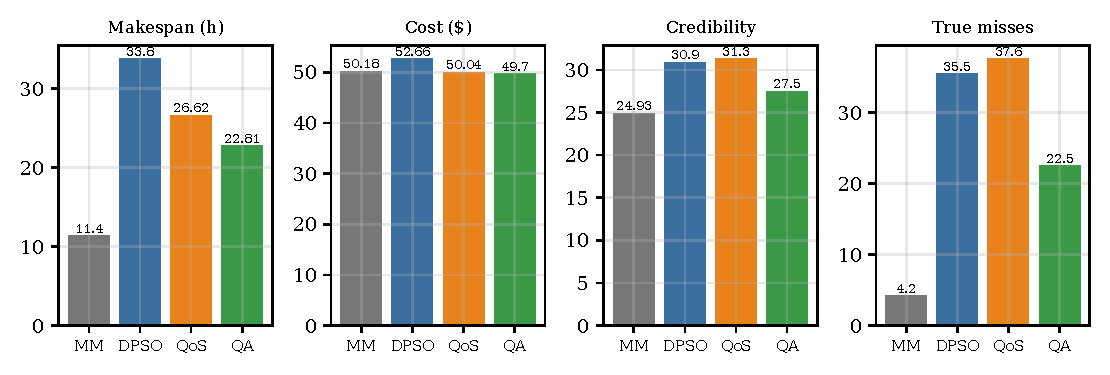
\includegraphics[width=0.95\textwidth]{fig_default.pdf}
\caption{Default setting ($n=100$, $l=4\times10^6$ MI), mean $\pm$ std over 10 seeds (MM = Min-Min, QoS = QoS-MDPSO, QA = QA-QoS-MDPSO, ours). The queue-aware fitness cuts makespan and true deadline misses relative to QoS-MDPSO.}\label{fig:default}
\end{figure}

\begin{table}[!t]
\caption{Mean over all settings and seeds. MS = makespan; TC = total credibility; True = queue-aware deadline misses; Eq.~9 = misses counted by the base paper's check; Bud.\ = budget misses; Fit.\ = paper fitness; Time = runtime per run}\label{tab:means}
\footnotesize
\setlength{\tabcolsep}{4pt}
\begin{tabular}{@{}lcccccccc@{}}
\toprule
Algorithm & MS (h) & TEC (\$) & TC & True & Eq.~9 & Bud. & Fit. & Time (s)\\
\midrule
\multicolumn{9}{@{}l}{\emph{Task-length sweep (80 runs per algorithm)}}\\
Min-Min & 25.48 & 112.7 & 25.0 & 47.0 & 2.76 & 25.6 & 37.30 & 0.001\\
DPSO & 67.89 & 116.4 & 29.2 & 56.1 & 6.86 & 32.2 & 51.21 & 0.064\\
QoS-MDPSO & 59.49 & 110.6 & 30.7 & 60.9 & 2.92 & 22.9 & 43.23 & 0.195\\
QA (ours) & 56.95 & 112.5 & 28.0 & 50.7 & 3.60 & 22.9 & 46.48 & 0.198\\
\midrule
\multicolumn{9}{@{}l}{\emph{Task-count sweep (50 runs per algorithm)}}\\
Min-Min & 9.32 & 39.6 & 19.1 & 3.8 & 0.34 & 17.8 & 9.60 & 0.001\\
DPSO & 24.38 & 41.3 & 23.5 & 22.7 & 1.26 & 24.3 & 13.47 & 0.057\\
QoS-MDPSO & 22.57 & 39.2 & 23.2 & 26.7 & 0.46 & 16.9 & 10.95 & 0.181\\
QA (ours) & 19.12 & 38.7 & 20.4 & 15.5 & 0.44 & 13.7 & 11.50 & 0.183\\
\bottomrule
\end{tabular}
\end{table}

\subsection{The deadline-check gap (RQ2)}\label{sec7.2}
The paper's Eq.~9 count and the true queue-aware count differ by one to two orders of magnitude (Table~\ref{tab:means}, Fig.~\ref{fig:len}). For QoS-MDPSO, Eq.~9 counts 2.9 misses per schedule in the length sweep and 0.46 in the count sweep, while the true counts are 60.9 and 26.7. At the default setting Eq.~9 reports 0.6 misses where 37.6 of 100 tasks actually finish late. An algorithm optimized with Eq.~9 therefore has almost no pressure to meet deadlines. For long tasks the deadlines become unattainable for every method (about 70 or more true misses at $l\ge12\times10^6$ MI, Table~\ref{tab:A1}), because the total work exceeds what 12 VMs can finish within about $4\times10^4$~s.

\begin{figure}[!t]
\centering
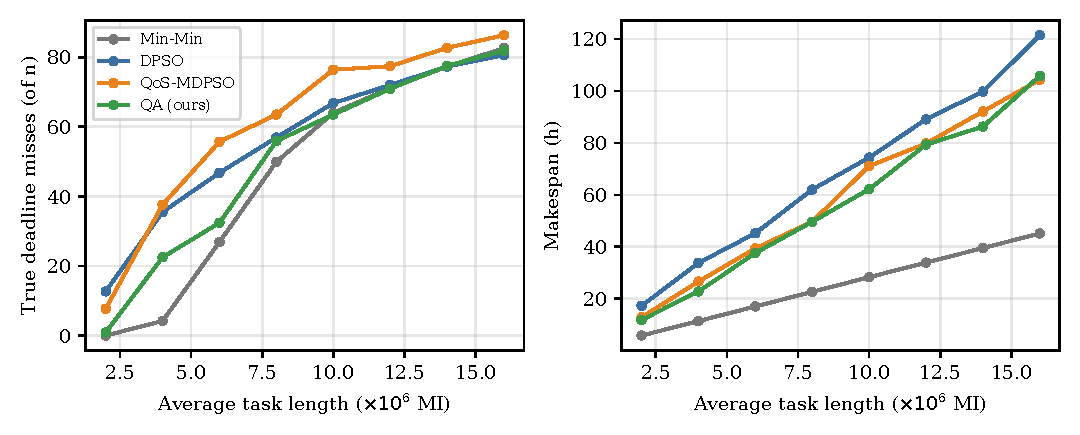
\includegraphics[width=\textwidth]{fig_len.pdf}
\caption{Task-length sweep (mean of 10 seeds). The panel of Eq.~9 counts (bottom middle) lies far below the true-miss panel (bottom left). Values are listed in Tables~\ref{tab:A1} and~\ref{tab:A2}.}\label{fig:len}
\end{figure}

\subsection{Effect of the queue-aware fitness}\label{sec7.3}
QA-QoS-MDPSO has the same search as QoS-MDPSO, so the differences in Table~\ref{tab:qa} come from the fitness alone. True deadline misses fall by 27.4\% in the length sweep and 58.9\% in the count sweep, both highly significant, and makespan falls by 5.6\% and 17.1\%. The median paired reduction in true misses is 7 tasks (length) and 8 tasks (count). The improvement percentages of Table~\ref{tab:qa} are averages over the settings of each sweep of the per-setting percentage change, so they differ from the ratio of the overall means in Table~\ref{tab:means}; the $p$-values come from Wilcoxon tests on the paired runs.

\begin{table}[!t]
\caption{QA-QoS-MDPSO relative to QoS-MDPSO (positive = better for us); Wilcoxon signed-rank on paired runs (80 length, 50 count)}\label{tab:qa}
\footnotesize
\begin{tabular}{@{}lcccc@{}}
\toprule
 & \multicolumn{2}{c}{Length} & \multicolumn{2}{c}{Count}\\
\cmidrule(lr){2-3}\cmidrule(lr){4-5}
Metric & Impr. & $p$ & Impr. & $p$\\
\midrule
True deadline misses & $+27.37\%$ & $1.2\times10^{-10}$ & $+58.94\%$ & $4.4\times10^{-6}$\\
Makespan & $+5.62\%$ & $4.3\times10^{-2}$ & $+17.06\%$ & $1.2\times10^{-3}$\\
Total credibility & $-8.30\%$ & $3.9\times10^{-6}$ & $-11.70\%$ & $4.3\times10^{-7}$\\
Cost & $-1.17\%$ & $6.4\times10^{-3}$ & $+1.26\%$ & $2.6\times10^{-1}$\\
Budget misses & $-1.70\%$ & $5.3\times10^{-1}$ & $+22.30\%$ & $2.5\times10^{-2}$\\
\bottomrule
\end{tabular}
\end{table}

At the default setting QA cuts true misses from 37.6 to 22.5 and makespan from 26.6~h to 22.8~h at a similar cost (\$49.7 against \$50.0). The price is credibility, which falls from 31.3 to 27.5 because the penalty pushes tasks to fast VMs regardless of their credibility. This is a trade-off, not a free improvement. Cost and budget differences are small and, in the length sweep, mixed or not significant. Under the paper fitness QA scores worse (46.5 against 43.2 and 11.5 against 10.95), as expected for an algorithm optimizing a different objective. The advantage holds at every task count (Fig.~\ref{fig:cnt}, Table~\ref{tab:A1}).

\begin{figure}[!t]
\centering
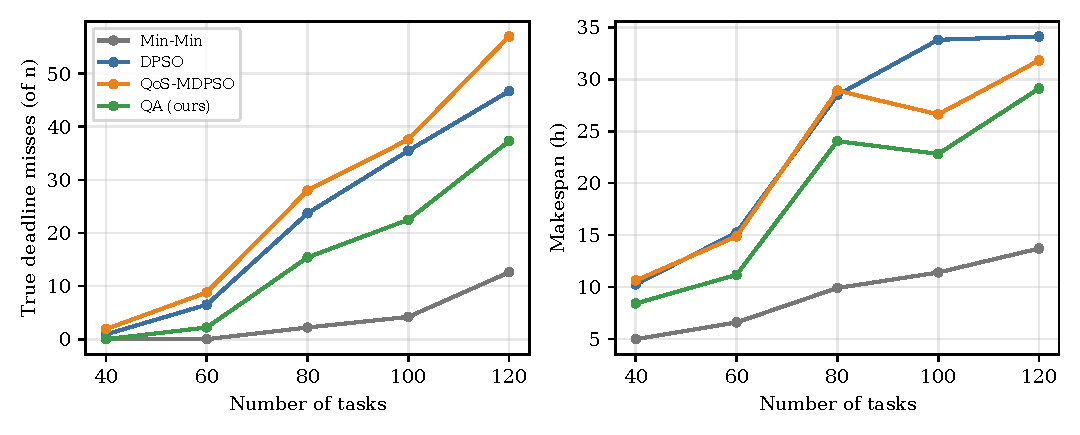
\includegraphics[width=\textwidth]{fig_cnt.pdf}
\caption{Task-count sweep (mean of 10 seeds). The queue-aware variant has the fewest true deadline misses among the PSO variants at every size.}\label{fig:cnt}
\end{figure}

\subsection{Penalty weight and convergence}\label{sec7.4}
The penalty weight sets the trade-off (Table~\ref{tab:lambda}, Fig.~\ref{fig:lambda}): raising $\lambda$ from 0.5 to 10 reduces true misses from 23.2 to 13.2 and budget misses from 26.2 to 16.1, while credibility falls from 27.3 to about 25--26. Makespan is not monotone in $\lambda$ (23.3, 22.8, 27.7, 26.8, 23.4~h); with 10 seeds the points are noisy, so $\lambda=1$ is a moderate default and no optimum is claimed.

\begin{table}[!t]
\caption{Sensitivity of QA-QoS-MDPSO to the penalty weight $\lambda$ (default setting, 10 seeds)}\label{tab:lambda}
\footnotesize
\begin{tabular}{@{}cccccc@{}}
\toprule
$\lambda$ & MS (h) & TEC (\$) & TC & True miss & Budget miss\\
\midrule
0.5 & 23.27 & 50.53 & 27.33 & 23.2 & 26.2\\
1 & 22.81 & 49.74 & 27.50 & 22.5 & 22.2\\
2 & 27.69 & 49.32 & 26.75 & 20.4 & 20.4\\
5 & 26.80 & 49.43 & 25.06 & 14.6 & 19.6\\
10 & 23.38 & 48.40 & 25.99 & 13.2 & 16.1\\
\bottomrule
\end{tabular}
\end{table}

\begin{figure}[!t]
\centering
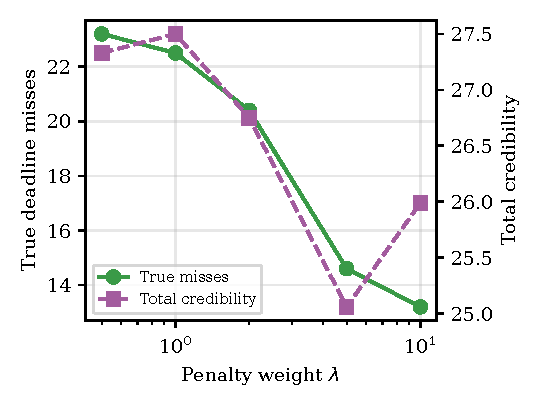
\includegraphics[width=0.5\textwidth]{fig_lambda.pdf}
\caption{Sensitivity to the penalty weight $\lambda$ (default setting, 10 seeds).}\label{fig:lambda}
\end{figure}

Under the paper's own fitness, QoS-MDPSO converges much faster than DPSO: in our 5-seed convergence runs its best fitness falls from about 25 to 11 within 35 iterations and ends near 10.2, against 13.6 for DPSO. It then stays almost flat for about 130 iterations, which suggests premature convergence. Part of its early lead reflects its larger number of fitness evaluations per iteration (Section~\ref{sec7.5}).

\begin{figure}[!t]
\centering
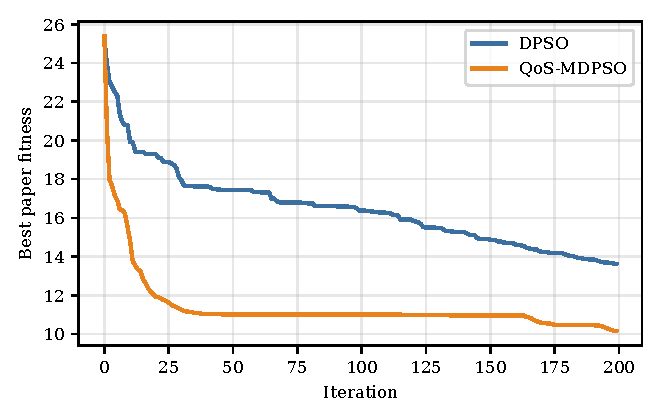
\includegraphics[width=0.55\textwidth]{fig_conv.pdf}
\caption{Convergence of the best paper fitness, mean of 5 seeds at the default setting.}\label{fig:conv}
\end{figure}

\subsection{Ablation of QoS-MDPSO (RQ3)}\label{sec7.5}
Each variant switches off exactly one mechanism and substitutes its DPSO counterpart: a linear inertia weight, the particle's own pbest, gbest, the plain update $X+V$, or no replacement. Table~\ref{tab:abl} and Fig.~\ref{fig:abl} show the results.

\begin{table}[!t]
\caption{Ablation (task-count sweep, 50 paired runs per variant, paper fitness). Change = relative change in mean paper fitness when the mechanism is removed (positive = removal hurts); $p$ = Wilcoxon versus full; Evals = fitness evaluations per run}\label{tab:abl}
\footnotesize
\setlength{\tabcolsep}{3.5pt}
\begin{tabular}{@{}lcccccccc@{}}
\toprule
Variant & Fit. & Change & $p$ & MS (h) & TEC & TC & True miss & Evals\\
\midrule
Full QoS-MDPSO & 10.950 & --- & --- & 22.57 & 39.18 & 23.19 & 26.7 & 18,030\\
no chaotic $w$ & 12.307 & $+12.39\%$ & $4.8\times10^{-3}$ & 21.53 & 40.40 & 23.22 & 18.4 & 18,030\\
no spbest & 10.295 & $-5.98\%$ & $5.8\times10^{-3}$ & 22.86 & 38.64 & 22.68 & 25.6 & 18,030\\
no mbest & 11.527 & $+5.27\%$ & $7.9\times10^{-3}$ & 27.58 & 38.75 & 23.02 & 30.7 & 18,030\\
no adaptive position & 12.757 & $+16.50\%$ & $8.8\times10^{-4}$ & 21.37 & 41.44 & 23.48 & 15.7 & 12,030\\
no worst replacement & 12.390 & $+13.14\%$ & $1.0\times10^{-3}$ & 27.72 & 38.75 & 22.08 & 33.9 & 12,030\\
all five off & 13.418 & $+22.54\%$ & $1.5\times10^{-8}$ & 23.60 & 41.23 & 22.92 & 21.1 & 6,030\\
\bottomrule
\end{tabular}
\end{table}

\begin{figure}[!t]
\centering
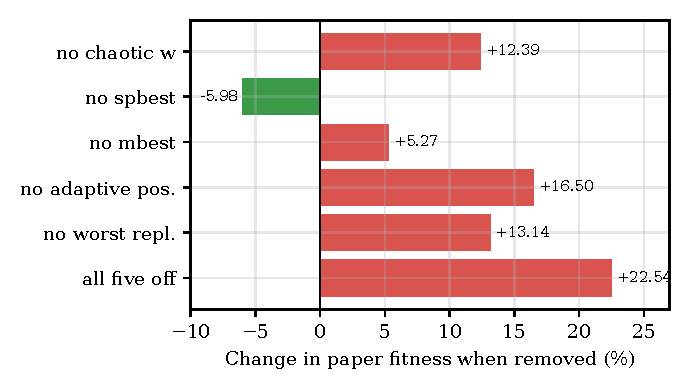
\includegraphics[width=0.62\textwidth]{fig_ablation.pdf}
\caption{Change in paper fitness when each mechanism is removed (positive = removal hurts).}\label{fig:abl}
\end{figure}

\begin{enumerate}
\item \textbf{Four mechanisms help the paper fitness; spbest does not.} Removing the chaotic weight, mbest, the adaptive position update or worst-particle replacement worsens the paper fitness by 5--17\%, and removing all five by 22.5\%. Removing spbest \emph{improves} it by 6.0\% ($p=0.006$): in our implementation the diversity-enhanced learning rule is harmful. This may depend on our assumed swarm size and iteration count.
\item \textbf{Evaluation budgets differ.} The full algorithm makes 18,030 fitness evaluations per run, 1.5$\times$ the variants without the adaptive update or replacement (12,030) and 3$\times$ the all-off variant (6,030), because those two steps each add a batch of evaluations per iteration. Their benefit is therefore confounded with a larger budget, and QoS-MDPSO is about three times slower than DPSO in our runs (0.18~s against 0.06~s in the count sweep), not ``similar'' as stated in \citet{ouyang2025}. The chaos, spbest and mbest ablations are budget-neutral.
\item \textbf{The paper fitness is a weak proxy for service quality.} The variant without the adaptive update has the worst paper fitness of the single-mechanism ablations, yet the lowest makespan (21.4~h) and the fewest true misses (15.7) of all variants; the variant without chaos behaves similarly. Since the paper fitness is dominated by cost in dollars, improvements in it do not imply better makespan or deadline compliance.
\item \textbf{Even the all-off variant is competitive} on makespan and true misses (23.6~h, 21.1), which suggests that much of the 22.5\% paper-fitness gain reflects the objective's structure rather than better search.
\end{enumerate}

\subsection{Credibility and failures (RQ4)}\label{sec7.6}
\paragraph{Credibility is predictive.} Over all 250 schedules in the paper scenario ($F\sim U(0,1)$), credibility per task correlates with the share of completed tasks at $r=0.889$. In the reliable scenario ($F\sim U(0.9,1)$) the correlation falls to 0.253 and every algorithm completes essentially all tasks (under 0.03 lost per schedule), so credibility stops mattering for completion (Fig.~\ref{fig:scatter}).

\begin{figure}[!t]
\centering
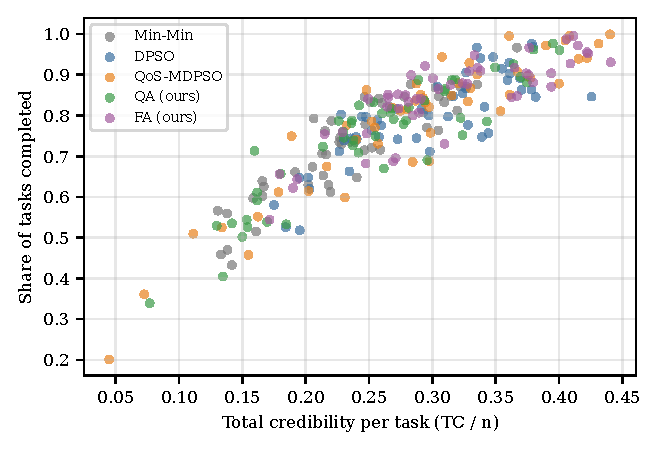
\includegraphics[width=0.55\textwidth]{fig_scatter.pdf}
\caption{Total credibility per task against the share of completed tasks, one point per schedule (paper scenario): $r=0.889$.}\label{fig:scatter}
\end{figure}

\begin{table}[!t]
\caption{Failure simulation, paper credibility range $F\sim U(0,1)$: mean over 50 runs $\times$ 200 scenarios. Done = share of tasks completed; Crit.-wt. = weighted by criticality; Lost crit. = lost tasks with $f\ge0.7$; Eff. = including re-runs; Late/lost = tasks lost or finishing after their deadline}\label{tab:fail}
\footnotesize
\setlength{\tabcolsep}{3.5pt}
\begin{tabular}{@{}lcccccccc@{}}
\toprule
Algorithm & TC & Done & Crit.-wt. done & Lost & Lost crit. & Eff. MS (h) & Eff. cost (\$) & Late/lost\\
\midrule
Min-Min & 19.06 & 0.727 & 0.723 & 21.6 & 7.03 & 25.06 & 74.0 & 37.0\\
DPSO & 23.45 & 0.796 & 0.820 & 16.4 & 4.17 & 51.15 & 71.0 & 43.8\\
QoS-MDPSO & 23.19 & 0.788 & 0.800 & 16.6 & 4.59 & 45.37 & 67.0 & 47.5\\
QA (ours) & 20.40 & 0.745 & 0.752 & 20.2 & 6.10 & 41.99 & 70.8 & 43.6\\
FA (ours) & 25.09 & 0.843 & 0.848 & 12.3 & 3.55 & 37.99 & 65.4 & 40.7\\
\bottomrule
\end{tabular}
\end{table}

\begin{figure}[!t]
\centering
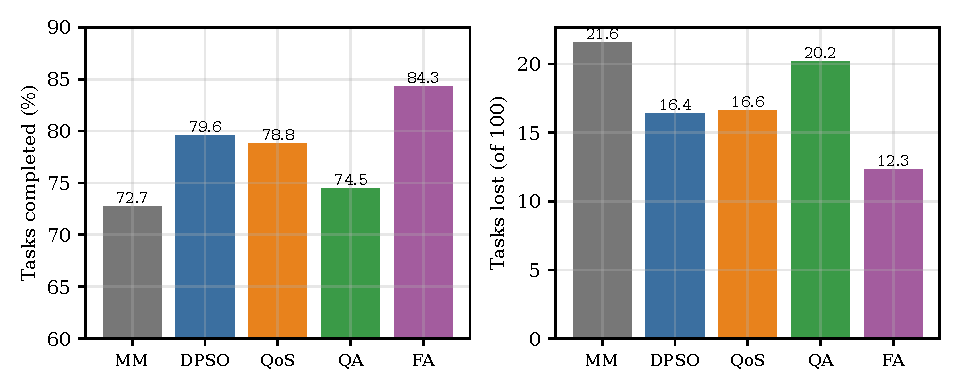
\includegraphics[width=\textwidth]{fig_fail.pdf}
\caption{Failure simulation with the paper's credibility range $U(0,1)$ (mean $\pm$ std, 50 runs $\times$ 200 scenarios; MM = Min-Min, QoS = QoS-MDPSO). FA completes the most tasks and loses the fewest.}\label{fig:fail}
\end{figure}

\paragraph{QA's weakness and FA's fix.} QA, which sacrifices credibility, completes fewer tasks than QoS-MDPSO (0.745 against 0.788, $p=6.7\times10^{-6}$; 3.6 more lost tasks) and loses more critical tasks (6.1 against 4.6), although it has fewer late-or-lost tasks ($-1.6$, $p=0.010$); its lower effective makespan is not significant ($p=0.16$). FA-QoS-MDPSO reverses this: relative to QoS-MDPSO it completes 3.4 percentage points more tasks ($p=1.5\times10^{-5}$), loses 2.6 fewer ($p=3.0\times10^{-5}$), and reduces the effective makespan by 6.6~h ($p=0.002$), the effective cost by \$1.1 ($p=0.022$) and late-or-lost tasks by 4.4 ($p=2.7\times10^{-6}$). Min-Min has the lowest effective makespan (25.1~h) and the fewest late-or-lost tasks (37.0), but loses the most tasks (21.6).

\paragraph{Reliable VMs.} When VMs are reliable the failure-related differences vanish and queueing dominates (Table~\ref{tab:rel}). Relative to QoS-MDPSO, QA reduces the effective makespan by 1.9~h ($p=9.9\times10^{-5}$) and late-or-lost tasks by 3.7 ($p=1.5\times10^{-6}$); FA is slightly better on late-or-lost tasks (15.6; $-2.6$, $p=4.8\times10^{-6}$), at about \$0.1 more cost ($p\approx0.05$). Min-Min remains clearly best here (11.2~h, 5.1 late or lost).

\begin{figure}[!t]
\centering
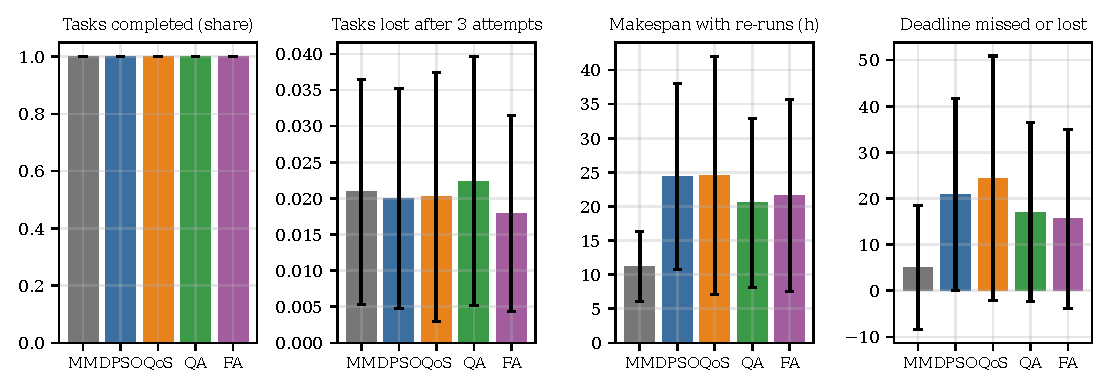
\includegraphics[width=\textwidth]{fig_rel.pdf}
\caption{Failure simulation with reliable VMs, $F\sim U(0.9,1)$. Completion is about 100\% for all methods; queueing dominates.}\label{fig:rel}
\end{figure}

\begin{table}[!t]
\caption{Failure simulation with reliable VMs, $F\sim U(0.9,1)$; columns as in Table~\ref{tab:fail}}\label{tab:rel}
\footnotesize
\setlength{\tabcolsep}{3.5pt}
\begin{tabular}{@{}lcccccccc@{}}
\toprule
Algorithm & TC & Done & Crit.-wt. done & Lost & Lost crit. & Eff. MS (h) & Eff. cost (\$) & Late/lost\\
\midrule
Min-Min & 38.31 & 1.000 & 1.000 & 0.021 & 0.007 & 11.19 & 41.7 & 5.1\\
DPSO & 38.40 & 1.000 & 1.000 & 0.020 & 0.006 & 24.40 & 42.6 & 20.8\\
QoS-MDPSO & 38.48 & 1.000 & 1.000 & 0.020 & 0.006 & 24.50 & 40.4 & 24.3\\
QA (ours) & 38.43 & 1.000 & 1.000 & 0.022 & 0.007 & 20.53 & 41.1 & 17.1\\
FA (ours) & 38.48 & 1.000 & 1.000 & 0.018 & 0.006 & 21.63 & 41.2 & 15.6\\
\bottomrule
\end{tabular}
\end{table}

%% ------------------------------------------------------------------
\section{Discussion}\label{sec8}
%% ------------------------------------------------------------------
\paragraph{What survives from the original paper.} The direction of the makespan and cost gains over DPSO, the faster convergence and the benefit of four of the five mechanisms are reproduced. The magnitudes differ, the credibility gain is not reproduced in the count sweep, and the ranking against Min-Min is reversed.

\paragraph{Why the evaluation model matters.} For QoS-MDPSO, 27--61 true misses per schedule against 0.5--3 counted by Eq.~9 show that the deadline constraint, as modelled in \citet{ouyang2025}, hardly affects optimization. The claim that QoS-MDPSO ensures tasks meet their deadlines is not supported under queue-aware evaluation, for either the original or our variant: at the default setting QA still leaves 22.5 of 100 tasks late, partly because the deadlines are tight relative to the total work.

\paragraph{Why makespan improves with the fix.} A task meets its deadline only if its VM's queue drains in time, so penalizing true misses pushes the swarm toward balanced loads, which also lowers the makespan. Eq.~9 provides no such pressure; it only rejects a task that is too long for a slow VM on its own. This observation is in line with the general importance of queueing and tail effects in large-scale services \citep{dean2013}.

\paragraph{Trade-offs are real.} QA's deadline and makespan gains are paid for with credibility, which the failure experiment shows costs completed tasks when VMs are unreliable; with reliable VMs, credibility is not worth trading against timeliness. FA-QoS-MDPSO, which uses credibility through expected attempts and losses, is the most robust PSO variant in our experiments.

\paragraph{Min-Min.} A credibility-blind completion-time heuristic beats all PSO variants on makespan and true misses in about a millisecond. PSO variants are justified only if cost and credibility are valued; seeding the swarm with the Min-Min schedule is an obvious hybrid that we did not test.

\subsection{Limitations and threats to validity}\label{sec8.1}
\begin{itemize}
\item \textbf{Synthetic data} following the paper's parameters; nothing was run on a real cloud or a trace.
\item \textbf{Assumed parameters:} swarm size, iterations, weights, budgets, the round-and-clip discretization and the failure model (success probability $F_j$, retries on the same VM, three attempts, independent failures). The spbest finding in particular may change with them.
\item \textbf{Simple queue model:} EDF order inside each VM for all algorithms, independent tasks, no data transfer, start-up delays or correlated failures. FIFO order would raise every method's true misses.
\item \textbf{Statistics:} 10 seeds per setting, uncorrected $p$-values, and large standard deviations across seeds; the paired tests treat (setting, seed) pairs as independent.
\item \textbf{Different objectives:} QA and FA optimize different functions from the paper fitness, so comparisons on the paper fitness favour QoS-MDPSO by construction; we report each metric separately.
\item \textbf{Equal iterations, not equal evaluations:} QoS-MDPSO and the full ablation variants receive more fitness evaluations than DPSO and the reduced variants.
\end{itemize}

%% ------------------------------------------------------------------
\section{Conclusion and future work}\label{sec9}
%% ------------------------------------------------------------------
A queue-aware re-evaluation shows that the deadline handling of QoS-MDPSO is largely ineffective: its check counts under 3 misses per schedule where 27--61 tasks actually finish late. Replacing only the fitness with a normalized, queue-aware one cuts true misses by 27--59\% and makespan by 6--17\%, at the price of 8--12\% of total credibility that a single weight controls. A failure simulation shows that credibility is meaningful ($r=0.889$ with task survival) when VMs are unreliable, that sacrificing it costs completed tasks, and that a failure-aware fitness recovers the loss (84.3\% of tasks completed against 78.8\% for QoS-MDPSO). The ablation indicates that four of the five mechanisms improve the paper fitness, that spbest does not, and that part of the gain stems from more fitness evaluations. A textbook Min-Min remains the strongest method on time-based objectives.

\textbf{Future work.} (1) Seed the swarm with the Min-Min schedule. (2) Compare all methods at equal numbers of fitness evaluations. (3) Use a permutation- or probability-based encoding that does not treat VM indices as numbers. (4) Model correlated failures and retries on other VMs. (5) Extend to workflows with dependencies, dynamic task arrivals and real traces, and validate on CloudSim \citep{calheiros2011} or a real cloud platform.

\backmatter

\bmhead{Supplementary information}
The per-setting results behind Figs.~\ref{fig:len} and~\ref{fig:cnt} are given in Appendix~\ref{secA1}. All CSV result files, statistics and figures are regenerated by the scripts in the project repository.

\bmhead{Acknowledgements}
The authors thank the course instructors of the Cloud Computing course at Netaji Subhas University of Technology, Main Campus, for guidance during this project.

\clearpage
\section*{Declarations}
\begin{itemize}
\item \textbf{Funding:} Not applicable.
\item \textbf{Conflict of interest/Competing interests:} The authors declare that they have no competing interests.
\item \textbf{Ethics approval and consent to participate:} Not applicable.
\item \textbf{Consent for publication:} Not applicable.
\item \textbf{Data availability:} All data are synthetic and generated by seeded scripts. The raw per-run result files (CSV) and the statistics reported in this paper are available in the \texttt{results} folder of the project repository (see Code availability).
\item \textbf{Materials availability:} Not applicable.
\item \textbf{Code availability:}\label{sec:avail} \url{https://github.com/Kanishk77295/QA-FA-QoS-MDPSO} (public repository containing the source code, implementation details, results, figures and the LaTeX source of this paper). Every parameter is defined once in \texttt{config.py} and marked PAPER or ASSUMED, every run is seeded, and the complete results are regenerated with \texttt{run\_experiments.py}, \texttt{run\_extensions.py}, \texttt{analyze.py} and \texttt{analyze\_extensions.py}.
\item \textbf{Author contribution:} All authors contributed equally to the implementation, experiments, analysis and writing.
\end{itemize}

\begin{appendices}

\section{Per-setting results}\label{secA1}
Tables~\ref{tab:A1} and~\ref{tab:A2} give the per-setting means behind Figs.~\ref{fig:len} and~\ref{fig:cnt}.

\begin{table}[!h]
\caption{True (queue-aware) deadline misses per setting, mean of 10 seeds}\label{tab:A1}
\footnotesize
\begin{tabular}{@{}lcccc@{}}
\toprule
Setting & Min-Min & DPSO & QoS-MDPSO & QA (ours)\\
\midrule
\multicolumn{5}{@{}l}{\emph{Task length ($\times10^6$ MI)}}\\
2 & 0.0 & 12.7 & 7.7 & 0.9\\
4 & 4.2 & 35.5 & 37.6 & 22.5\\
6 & 26.9 & 46.8 & 55.7 & 32.4\\
8 & 49.9 & 56.9 & 63.5 & 55.9\\
10 & 64.0 & 66.8 & 76.4 & 63.5\\
12 & 71.1 & 72.0 & 77.4 & 70.9\\
14 & 77.3 & 77.3 & 82.7 & 77.5\\
16 & 82.6 & 80.6 & 86.3 & 81.9\\
\midrule
\multicolumn{5}{@{}l}{\emph{Number of tasks}}\\
40 & 0.0 & 0.9 & 1.9 & 0.0\\
60 & 0.0 & 6.5 & 8.8 & 2.2\\
80 & 2.2 & 23.7 & 28.0 & 15.4\\
100 & 4.2 & 35.5 & 37.6 & 22.5\\
120 & 12.6 & 46.7 & 57.0 & 37.3\\
\bottomrule
\end{tabular}
\end{table}

\begin{table}[!h]
\caption{Makespan (h) per setting, mean of 10 seeds}\label{tab:A2}
\footnotesize
\begin{tabular}{@{}lcccc@{}}
\toprule
Setting & Min-Min & DPSO & QoS-MDPSO & QA (ours)\\
\midrule
\multicolumn{5}{@{}l}{\emph{Task length ($\times10^6$ MI)}}\\
2 & 5.82 & 17.25 & 12.85 & 11.81\\
4 & 11.40 & 33.80 & 26.62 & 22.81\\
6 & 17.03 & 45.23 & 39.39 & 37.60\\
8 & 22.66 & 62.06 & 49.68 & 49.64\\
10 & 28.31 & 74.39 & 71.11 & 62.19\\
12 & 33.93 & 89.09 & 79.79 & 79.38\\
14 & 39.54 & 99.81 & 92.13 & 86.32\\
16 & 45.14 & 121.49 & 104.36 & 105.83\\
\midrule
\multicolumn{5}{@{}l}{\emph{Number of tasks}}\\
40 & 4.98 & 10.25 & 10.63 & 8.42\\
60 & 6.60 & 15.26 & 14.88 & 11.18\\
80 & 9.91 & 28.48 & 28.91 & 24.05\\
100 & 11.40 & 33.80 & 26.62 & 22.81\\
120 & 13.71 & 34.12 & 31.81 & 29.11\\
\bottomrule
\end{tabular}
\end{table}

\end{appendices}

\bibliography{references}

\end{document}
